%%%%%%%%%%%%%%%%%%%%% chapter.tex %%%%%%%%%%%%%%%%%%%%%%%%%%%%%%%%%
%
% sample chapter
%
% Use this file as a template for your own input.
%
%%%%%%%%%%%%%%%%%%%%%%%% Springer-Verlag %%%%%%%%%%%%%%%%%%%%%%%%%%
%\motto{Use the template \emph{chapter.tex} to style the various elements of your chapter content.}
\chapter{An Overview on ETSI’s LBT Mechanisms}
\label{sec:LBT-overview} 

%TODO: Abstract
\abstract{Each chapter should be preceded by an abstract (10--15 lines long) that summarizes the content. The abstract will appear \textit{online} at \url{www.SpringerLink.com} and be available with unrestricted access. This allows unregistered users to read the abstract as a teaser for the complete chapter. As a general rule the abstracts will not appear in the printed version of your book unless it is the style of your particular book or that of the series to which your book belongs.\newline\indent
Please use the 'starred' version of the new Springer \texttt{abstract} command for typesetting the text of the online abstracts (cf. source file of this chapter template \texttt{abstract}) and include them with the source files of your manuscript. Use the plain \texttt{abstract} command if the abstract is also to appear in the printed version of the book.}


\section{Radio Spectrum and Its Allocation}

The radio spectrum is the part of the electromagnetic spectrum from $3$ Hz to $3000$ GHz ($3$ THz). Radio waves in this frequency range are widely used in modern technologies, especially in telecommunications. The radio spectrum is divided into different chunks or bands, each of which can be used by one or multiple technologies. Radio Frequency Interference (RFI) is the conduction or radiation of radio frequency energy that causes an electronic or electrical device to produce unwanted noise that typically interferes with functions of adjacent devices.  In radio communications, RFI can disrupt and disturb the normal functioning of devices, and thus it is always important to avoid or keep the RFI within acceptable levels. In order to prevent RFI, the generation and transmission of radio waves is strictly regulated by national laws, coordinated by international organizations, e.g., International Telecommunication Union (ITU), European Conference of Postal and Telecommunications Administrations (CEPT), Inter-American Telecommunication Commission (CITEL), European Telecommunications Standards Institute (ETSI), etc. 

It most countries, the use of radio frequency bands is regulated by national radio allocation authorities. Spectrum allocation varies by country and/or regulatory domain. In United States, for example, the Federal Communications Commission (FCC) regulates inter-state communications by radio, television, wire, satellite, and cable in all states and territories. From management perspectives, radio bands are categorized into licensed and unlicensed. Licensing is a way of ensuring that wireless operators do not interfere with each others by giving each of them an exclusive use of given bands in given geographical areas over a set period of time. Licensed bands are mainly sold/assigned to operators through spectrum auction precess. They are mainly used by television broadcasting, commercial radio and cellular voice and data. Operating in licensed bands, mobile cellular networks can avoid RFI and thus guarantee quality of services to their subscribers. However, licensing would be very impractical for certain uses, like communications between cordless handsets and base units. Instead, such a kind of wireless technology transmits in unlicensed frequency bands - usually the Industrial, Scientific and Medical (ISM) band defined by the ITU radio regulations and allocated in most countries for free use by anyone without any license and fee. Unlicensed bands enable numerous technologies and products, e.g., Wi-Fi, Bluetooth, and many other low-power short-range communications technologies. They are also open sandboxes where users can operate without the high barriers to entry. They provide a platform for innovation, a greenfield space for technology start-ups and entrepreneurs and established companies. Internet of Things (IoT) - the development and deployment of networking technologies that provide connectivity for everyday objects for many innovative applications - is essentially enabled by unlicensed spectrum.

There is a considerable amount of unlicensed spectrum. $2.4$ and $5$ GHz are the two most widely used unlicensed bands. Today, most people are within a few meters of consumer products (microwave ovens, Wi-Fi, Bluetooth, etc.) that use these bands. In other words, there is a great chance for RFI. As a result, even though no permission is required for the use of unlicensed bands, manufacturers and users of devices must comply with numerous rules and regulations (related to transmission power, transmission time, etc.) in order to minimize the RFI to others in these bands as well as to ensure a fair sharing of the radio resource. IEEE 802.11/Wi-Fi is the most successful and popular technology operating in unlicensed spectrum. Wi-Fi manufacturers need to obtain compliance certifications from Wi-Fi Alliance whose certification program is designed following rules imposed by radio spectrum management organizations/authorities such as ETSI and FCC. 

New technologies, particularly unlicensed LTE variants including LTE-U, LAA, and MulteFire (as mentioned in chapter xx), have been developed to operate in the $5$ GHz unlicensed spectrum alongside Wi-Fi. The $5$ GHz band is more often selected for new technologies rather than the $2.4$ GHz band due to the following reasons:
\begin{itemize}
\item
More available channels: In the $2.4$ GHz band, only $13$ channels are available. Moreover, these channels overlap excessively with one another. Due to this overlapping, the maximum possible
number of parallel independent connections is limited to $3$ channels. 
\item
Lower level of interference: Since the $2.4$ ISM band has been released for use for many years, a great number of radio applications have been established for this band. As such, the 802.11b/g standard WLANs are often forced to compete with interference from these applications. In contrast, the relatively recent release of the $5$ GHz band for private use gives WLAN usage a very prominent position in this frequency range. Other than military applications, which are isolated from 802.11a/h by special mechanisms, there are virtually no sources of interference. 
\item
Higher performance: The $5$ GHz band allows for significantly higher performance than the $2.4$ GHz band. This makes $5$ GHz band WLANs much better suited for outdoor applications and directional radio connections (point-to-point) than wireless connections in the $2.4$ GHz band. 
\end{itemize}

It is imperative to ensure that U-LTE devices comply with unlicensed band rules and regulations in order to limit the RFI that this technology may introduce to Wi-Fi devices/networks currently used by billions of users every day in homes, offices, and buildings. Since the number of wireless devices using the $5$GHz band has grown rapidly over the last few years, ETSI has updated its related standards. For background knowledge necessary for the development of radio channel access protocol in this band, the following sections summarize a number of key requirements presented in ETSI EN 301 893 V1.7.2 regulations \cite{LBT-ETSI-2014} released in July 2014.

\begin{figure}[!t]
	\centering
	\includegraphics[width=1.0\columnwidth]{figures2/5GHz-spectrum.pdf}
	\caption{$5$ GHz Unlicensed Spectrum.}
	\label{figs:5GHz-spectrum}
\end{figure}


\section{Frequency Bands}

To standardize the use of the $5$ GHz band in Europe, the European Commission issued the ETSI 301 893 standard on July 11, 2005. The member states of the EU were obliged to implement this by October 31, 2005. The ETSI 301 893 standard regulates three frequency bands with different specifications:
\begin{itemize}
\item
RLAN band 1: $5150$ to $5350$ MHz, divided into 2 sub-bands
\begin{itemize}
\item
Sub-band I: $5150$ MHz - $5250$ MHz (channels 36, 40, 44 and 48) 
\item
Sub-band II: $5250$ MHz - $5350$ MHz (channels 52, 56, 60 and 64) 
\end{itemize}
\item
RLAN band 2: $5470$ MHz - $5725$ MHz (channels 100, 104, 108, 112, 116, 120, 124, 128, 132, 136 and 140)
\item
RLAN band 3, also known as Broadband Radio Access Networks (BRAN): $5725$ – $5875$ MHz (channels 147, 151, 155 and 167, may only be used in Great Britain)
\end{itemize}

Fig. \ref{figs:5GHz-spectrum} summarizes radio channels defined in the $5$ GHz band by ETSI 301 893 standard (with a reference to FCC regulations). Technical details and the availability of each channel in four main regions (U.S., Europ, Japan, and China) are presented in Fig. \ref{figs:5GHz-spectrum-table}.

\begin{figure}[!t]
	\centering
	\includegraphics[width=0.85\columnwidth]{figures2/5GHz-spectrum-table.pdf}
	\caption{Details of $5$ GHz Unlicensed Channels in Different Regions.}
	\label{figs:5GHz-spectrum-table}
\end{figure}


\section{Transmission Power}

As presented in previous section, the $5$ GHz band is divided into three different ETSI RLAN bands. Each of these three bands have different power limits. Note that the RF output power is defined as the mean Equivalent Isotropic Radiated Power (EIRP) of the equipment during a transmission burst. In general, the limits are valid for the device with antenna gain and cable loss and not only the output power of WLAN module.

\subsection{RLAN band 1 ($5150$ to $5350$ MHz)}

\subsubsection{Indoor only Sub-band I ($5150$ - $5250$ MHz)}
The first RLAN sub-band includes the channels $36$ to $48$ and has an EIRP power limit to $23$ dBm ($200$ mW). These channels are considered for indoor only usage and do not require any Dynamic Frequency Selection (DFS) or Transmit Power Control (TPC) features. It is comparable to FCC U-NII-1.

\subsubsection{Indoor only Sub-band II ($5250$ - $5350$ MHz)}
In the second sub-band of the RLAN band 1 with channels $52$ to $64$, the ETSI has set the EIRP power limit to $23$ dBm ($200$ mW) for devices with TPC and $20$ dBm ($100$ mW) for devices without TPC. For a device with TPC, the mean EIRP at the lowest power level of the TPC range must not exceed $17$ dBm ($50$ mW). This band requires DFS support and is comparable to FCC U-NII-2.

\subsection{RLAN band 2 ($5470$ to $5725$ MHz)}

Channels from $100$ to $140$ are part of the second RLAN band and have an EIRP power limit of $30$ dBm ($1000$ mW) for TPC and $27$ dBm ($500$ mW) for non-TPC devices or $20$ dBm ($100$ mW) for devices without any TPC or DFS support. The mean EIRP power level for a slave device with TPC must not exceed $24$ dBm at the the lowest TPC power level if the device is also capable of radar detection or $17$ dBm otherwise. This band can be used for in- and outdoor deployments as well and is comparable to FCC U-NII-2e.

\subsection{BRAN ($5725$ to $5875$ MHz)}

Comparable to the FCC U-NII-3 ($5725$ – $5825$ MHz) band with a higher upper frequency range, the ETSI has defined the channels $155$ to $171$ (155, 159, 163, 167, 172) for Broadband Wireless Access (BWA) use only. The idea is to give internet access to locations without any wired access network available. The maximum EIRP output power has been set to $36$ dBm ($4000$ mW) with the limitation of RF power into antenna of $304$ dBm ($1000$ mW).


\section{Spectrum Access Requirements}
\label{subsec:ETSI-overview}

ETSI describes a number of spectrum access mechanisms to facilitate spectrum sharing for wireless access systems in $5$ GHz frequency band. This sections focuses on Dynamic Frequency Selection (DFS), Transmission Power Control (TPC), and Listen Before Talk (LBT)

\subsection{Dynamic Frequency Selection (DFS)}

DFS was stipulated to prioritize primary applications. DFS initially assumes that no channel is available in the corresponding frequency band. The WLAN device selects an arbitrary channel at the start and performs what is known as a Channel Availability Check (CAC). Before sending to a channel for 60 seconds (Channel Observation Time, COT), a check is run to see if a different device is already working on this channel and the channel is therefore occupied. If this is the case, then a different channel is checked by the CAC. If not, then the WLAN device can perform the transmission operation. Even during operation, a check is run to see if a primary application such as a radar device is using this channel. This exploits the fact that radars frequently work according to the rotation method, whereby a tightly bundled directional transmission signal is transmitted by a rotating antenna. A remote receiver perceives the radar signal as a short pulse (radar peak). If a device receives such a radar peak, it pauses the transmission operation and monitors the channel for further pulses. If additional radar peaks occur during the COT, then a new channel is selected automatically. A check of this type is required to be carried out every 24 hours. This is why interrupting the data transmission for 60 seconds is unavoidable. DFS is stipulated for the frequency ranges of 5250 - 5350 MHz and from 5470 - 5725
MHz. It is optional for the frequency range of 5150 - 5250 MHz. 

\subsection{Transmission Power Control (TPC)}
Dynamic adjustment of the transmission power is intended to reduce radio interference. Dynamically adjusting the transmission power facilitates the shared use of the 5250-5350 MHz and 5470 - 5725 MHz frequency bands with satellite services. TPC should cause an average reduction in the transmission power by at least 3 dB compared with the maximum permitted transmission power. TPC determines the minimum transmission power necessary to maintain the connection with the partner (such as an access point). If TPC is not used within these frequency bands, then the highest permissible average EIRP and the corresponding maximum EIRP density are reduced by 3 dB. This restriction does not apply to the frequency range of 5150 - 5350 MHz. Without DFS and TPC, a maximum of only 30 mW EIRP is permitted. When DFS and TPC are used, a maximum 1000 mW EIRP is permitted as the transmission power (compared with 100 mW with 802.11 b/g, 2.4 GHz, DFS and TPC are not possible here). The higher maximum transmission
power not only compensates for the higher attenuation of 5 GHz radio waves in air, it also makes noticeably longer ranges possible than in the 2.4 GHz range. 

\subsection{Listen Before Talk (LBT)}

LBT describes two machanisms that require an equipment or a device to apply CCA before using the channel to avoid collisions. The first mechanism is Frame Based Equipment (FBE) which defines a fixed (not directly demand-driven) timing frame for channel access. The second mechanism is Load Based Equipment (LBE) which defines demand-driven timing frame.

\begin{figure}[!t]
	\centering
	\includegraphics[width=0.9\columnwidth]{figures2/FBE-flowchart}
	\caption{Simplified flowchart of FBE.}
	\label{figs:FBE-flowchart}
\end{figure}

\begin{figure}[!t]
	\centering
	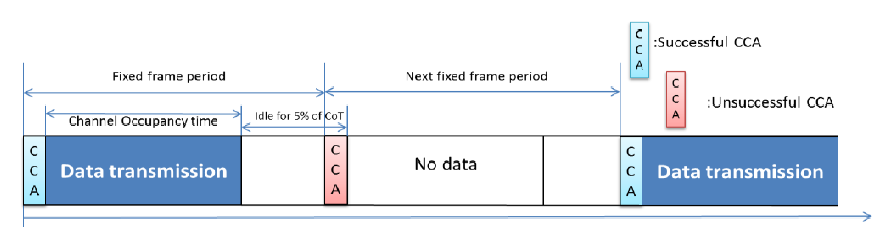
\includegraphics[width=0.9\columnwidth]{figures2/FBE-example}
	\caption{An illustrative example of FBE.}
	\label{figs:FBE-example}
\end{figure}


\subsubsection{FBE-based Mechanism}
\label{etsi-lbt:fbe}

FBE shall comply with the following requirements:

\begin{itemize}
	
	\item
	\textit{R1:} Before starting transmissions on an operating channel, the equipment shall perform a CCA check using Energy Detect (ED). The equipment shall observe the channel for the duration of the \textit{CCA observation time}. The operating channel shall be considered occupied if the energy level in the channel exceeds the \textit{threshold} corresponding to the power level.
	
	\item
	\textit{R2:}
	If the CCA procedure finds the channel clear, the equipment may transmit immediately and occupy the channel for a \textit{fixed time period}.
	
	\item
	\textit{R3:} If the CCA procedure finds the channel occupied, the equipment shall not transmit on that channel during the next fixed frame period.
	
	\item
	\textit{R4:} The total time during which an equipment has transmissions on a given channel without re-evaluating the availability of that channel is defined as the \textit{Channel Occupancy Time} (CoT).
	
	\item
	\textit{R5:} After occupying the channel for CoT, the equipment keeps silent and waits for a short time, namely \textit{Idle Period} (IP).
	
	\item
	\textit{R6:} Towards the end of the idle period, the equipment shall perform a new CCA procedure as described in R1 above.
	
	\item
	\textit{R7:} The equipment, upon correct reception of a packet which was intended for this equipment, can skip CCA and immediately proceed with the transmission of management and control frames, e.g., acknowledgment (ACK) and block ACK frames.
	
	\item
	\textit{R8:}
	A consecutive sequence of such transmissions by the equipment, without it performing a new CCA, shall not exceed the maximum CoT.
	
	\item
	\textit{R9:}
	CCA observation time shall be not less than $20$ $\mu$s.
	
	\item
	\textit{R10:} CoT shall be in the range from $1$ ms to $10$ ms.
	
	\item
	\textit{R11:}
	The minimum IP shall be at least $5$\% of CoT used by the equipment for the current fixed frame period.
	
\end{itemize}

A simplified flowchart and an illustrative of FBE are given in Figs. \ref{figs:FBE-flowchart} and \ref{figs:FBE-example}, respectively.


\begin{figure}[!t]
	\centering
	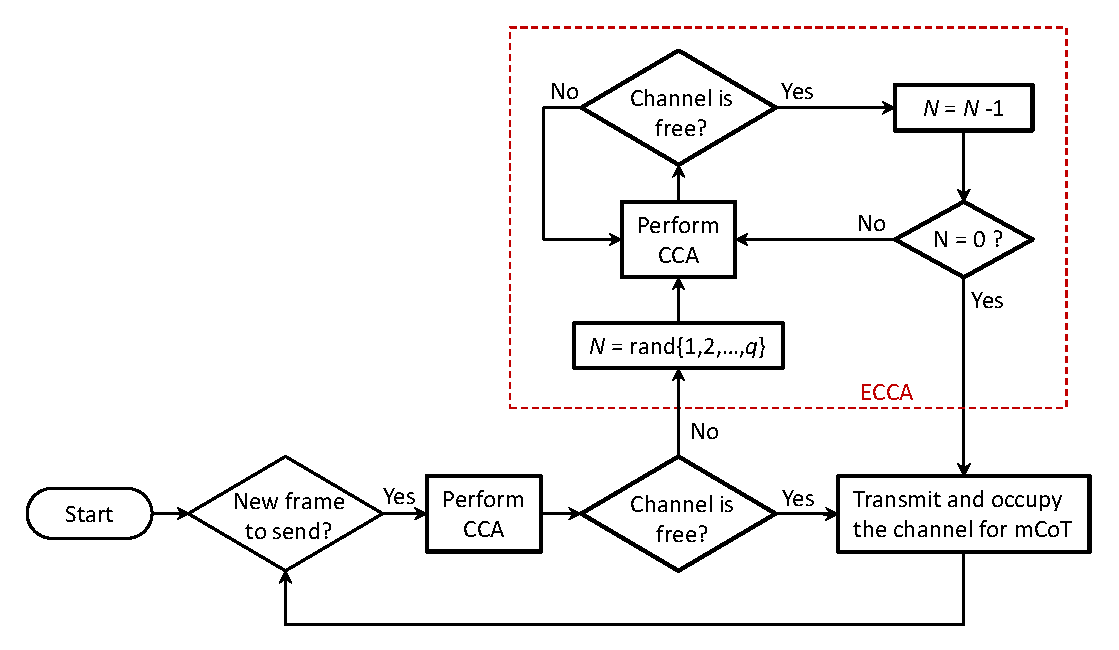
\includegraphics[width=0.9\columnwidth]{figures2/LBE-flowchart}
	\caption{Simplified flowchart of LBE.}
	\label{figs:LBE-flowchart}
\end{figure}

\begin{figure}[!t]
	\centering
	\includegraphics[width=0.9\columnwidth]{figures2/LBE-example}
	\caption{An illustrative example of LBE.}
	\label{figs:LBE-example}
\end{figure}


subsubsection{LBE-based Mechanism}
\label{etsi-lbt:lbe}

LBE shall comply with the following requirements:

\begin{itemize}
	
	\item
	\textit{R1:} Before starting transmissions on an operating channel, the equipment shall perform a CCA check using ED. The equipment shall observe the channel for the duration of the \textit{CCA observation time}. The operating channel shall be considered occupied if the energy level in the channel exceeds the threshold corresponding to the power level.
	
	\item
	\textit{R2:}
	If the CCA procedure finds the channel clear, the equipment may transmit immediately on that channel.
	
	\item
	\textit{R3:}
	If the CCA procedure finds the channel occupied, it shall not transmit in that channel. The equipment shall perform an Extended CCA (ECCA) procedure in which the channel is observed for a random duration.
	
	\item
	\textit{R4:}
	If the ECCA procedure has determined the channel to be clear, the equipment may start transmissions on this channel.
	
	\item
	\textit{R5:}
	The total time that an equipment makes use of the channel (without performing CCA) is the \textit{maximum Channel Occupancy Time} (mCoT), after which the device shall perform a new CCA procedure as described in R1 above.
	
	\item
	\textit{R6:}
	The equipment, upon correct reception of a packet which was intended for this equipment, can skip CCA and immediately proceed with the transmission of management and control frames, e.g., ACK and block ACK frames.
	
	\item
	\textit{R7:}
	A consecutive sequence of transmissions by the equipment, without it performing a new CCA, shall not exceed mCoT.
	
	\item
	\textit{R8:}
	CCA observation time shall be not less than $20$ $\mu$s.
	
	\item
	\textit{R9:}
	The random duration in an ECCA procedure is $N \times$ (CCA observation time), where $N$ is randomly selected in the range $\{1,2,...,q\}$, $q \in \{4,5,...,32\}$ (declared by the manufacturer).
	
	\item
	\textit{R10:}
	mCoT should be less than $(13/32)\times q$ ms (mCoT is in the range from $1.625$ to $13$ ms).
	
\end{itemize}

A simplified flowchart and an illustrative of LBE are given in Figs. \ref{figs:LBE-flowchart} and \ref{figs:LBE-example}, respectively.


\input{referenc-lbt}